% =====================================================================
% Yazılım Laboratuvarı-II, Proje I - Proje Raporu (IEEE konferans formatı)
% Derleme: pdflatex rapor.tex  (iki kez)   veya   latexmk -pdf rapor.tex
% Overleaf: Menu -> Compiler: pdfLaTeX
% =====================================================================
\documentclass[conference,a4paper]{IEEEtran}

\usepackage[T1]{fontenc}
\usepackage[utf8]{inputenc}
% shorthands=off: Türkçe paketinin "=" ve ":" karakterlerine verdiği özel
% anlamı kapatır (aksi halde \includegraphics[width=...] gibi ayarlar bozulur).
\usepackage[shorthands=off,turkish]{babel}
\usepackage{amsmath}
\interdisplaylinepenalty=2500
\usepackage{cite}
\usepackage{graphicx}
\usepackage{booktabs}
\usepackage{array}
\usepackage{url}
\usepackage{algorithm}
\usepackage[noend]{algpseudocode}
\usepackage{tikz}
\usetikzlibrary{babel,positioning,arrows.meta}

% --- IEEEtran'ın İngilizce sabit metinlerini Türkçeleştirme -------------
\addto\captionsturkish{\renewcommand{\IEEEkeywordsname}{Anahtar Kelimeler}}
\floatname{algorithm}{Algoritma}
\algrenewcommand\algorithmicrequire{\textbf{Girdi:}}
\algrenewcommand\algorithmicensure{\textbf{Çıktı:}}
\algrenewcommand\algorithmicif{\textbf{eğer}}
\algrenewcommand\algorithmicthen{\textbf{ise}}
\algrenewcommand\algorithmicelse{\textbf{değilse}}
\algrenewcommand\algorithmicfor{\textbf{her}}
\algrenewcommand\algorithmicdo{\textbf{için}}
\algrenewcommand\algorithmicreturn{\textbf{döndür}}
% Not: IEEEtran bölüm ve tablo başlıklarını büyük harfe çevirirken Türkçe
% "i" harfini noktasız "I" yapar. Bu yüzden bölüm ve tablo başlıkları
% doğrudan büyük harfle (İ ile) yazılmıştır.

\begin{document}

\title{Web Kazıma Tabanlı Kentsel Haber İzleme ve\\Harita Üzerinde Görselleştirme Sistemi}

\author{\IEEEauthorblockN{Burak Kılcı}
\IEEEauthorblockA{Bilgisayar Mühendisliği Bölümü\\
Kocaeli Üniversitesi\\
Öğrenci No: 230202111\\
230202111@kocaeli.edu.tr}

}

\maketitle

\begin{abstract}
Bu çalışmada, Kocaeli ilindeki beş yerel haber sitesinden trafik kazası, yangın,
elektrik kesintisi, hırsızlık ve kültürel etkinlik haberlerini otomatik olarak
toplayan, işleyen ve harita üzerinde gösteren bir sistem geliştirilmiştir. Sistem
Python ile yazılmış, veriler MongoDB'de saklanmıştır. Haber metinleri temizlenip
normalize edildikten sonra ağırlıklı anahtar kelime yöntemiyle sınıflandırılmış,
olay yeri kural tabanlı bir yöntemle metinden çıkarılarak koordinata
dönüştürülmüştür. Farklı sitelerde yayımlanan aynı haberler, çok dilli bir cümle
gömme (embedding) modeliyle ölçülen \%90 ve üzeri kosinüs benzerliği ile tespit
edilip tek kayıtta birleştirilmiştir. Gerçek verilerle yapılan ilk taramada 39
haber kaydedilmiş, 9 haber başka sitelerdeki kopyalarıyla birleştirilmiştir.
Sınıflandırma hatalarının analiziyle geliştirilen kurallar sonucunda yanlış
sınıflandırılan 15 haberin tamamı elenmiştir. Kalan haberlerin \%66,7'sinde olay
yeri ilçe merkezinden daha spesifik (mahalle, cadde veya belirli bir yer
düzeyinde) bulunmuştur.
\end{abstract}

\begin{IEEEkeywords}
web kazıma, haber sınıflandırma, konum çıkarımı, geocoding, cümle gömme,
MongoDB, harita görselleştirme
\end{IEEEkeywords}

% =====================================================================
\section{GİRİŞ}
Şehir yaşamını etkileyen trafik kazaları, yangınlar, elektrik kesintileri ve
kültürel etkinlikler gibi olaylar çok sayıda yerel haber sitesinde dağınık
biçimde yayımlanmaktadır. Bir kullanıcının çevresindeki olayları takip etmesi
için bu siteleri tek tek gezmesi gerekmekte, aynı olay farklı sitelerde farklı
başlıklarla tekrar karşısına çıkmaktadır. Ayrıca haber metinleri olayın yerini
çoğunlukla ``Körfez ilçesi Yeniyalı Mahallesi Cahit Zarifoğlu Caddesi'' gibi
serbest metin olarak verdiği için, olayların mekânsal dağılımını görmek mümkün
olmamaktadır.

Bu projede bu soruna yönelik uçtan uca bir sistem geliştirilmiştir. Sistem;
(i)~belirlenen beş yerel siteden son üç günün haberlerini otomatik olarak
toplar, (ii)~metinleri temizler ve beş olay türünden birine atar, (iii)~metindeki
konum ifadelerini bularak koordinata dönüştürür, (iv)~farklı kaynaklardaki aynı
haberleri birleştirir ve (v)~sonuçları türüne göre renklendirilmiş işaretlerle
etkileşimli bir harita üzerinde sunar.

Raporun geri kalanı şöyle düzenlenmiştir: Bölüm~\ref{sec:mimari} sistem mimarisini,
Bölüm~\ref{sec:kazima}--\ref{sec:tekrar} her işlem adımını, Bölüm~\ref{sec:arayuz}
kullanıcı arayüzünü, Bölüm~\ref{sec:deney} gerçek verilerle elde edilen
sonuçları, Bölüm~\ref{sec:sorunlar} karşılaşılan sorunları ve
Bölüm~\ref{sec:sonuc} sonuçları ele almaktadır.

% =====================================================================
\section{SİSTEM MİMARİSİ}\label{sec:mimari}
Sistem Python~3.11 ile geliştirilmiştir. Kullanılan başlıca bileşenler şunlardır:
web kazıma için \texttt{requests} ve BeautifulSoup~\cite{bs4}, veritabanı için
MongoDB~\cite{mongodb}, zamanlanmış görevler için APScheduler~\cite{apscheduler},
benzerlik ölçümü için \texttt{sentence-transformers}~\cite{sbert} ve web sunucusu
için Flask~\cite{flask}. Arayüz HTML, CSS ve JavaScript ile yazılmıştır.

İşlem hattı Şekil~\ref{fig:mimari}'de gösterilmiştir. Bir tarama çalışmasında beş
site paralel olarak taranır. Toplanan haberler ardından tek tek temizleme,
sınıflandırma, Kocaeli kontrolü, benzerlik kontrolü, konum çıkarımı ve geocoding
adımlarından geçirilir. Bir haber herhangi bir adımda elenirse (ör. hiçbir türe
girmiyorsa) bu sonuç nedeniyle birlikte kaydedilir ve haber sonraki adımlara
geçmez. MongoDB'de kullanılan koleksiyonlar Tablo~\ref{tab:koleksiyon}'da
verilmiştir.

\begin{figure*}[!t]
\centering
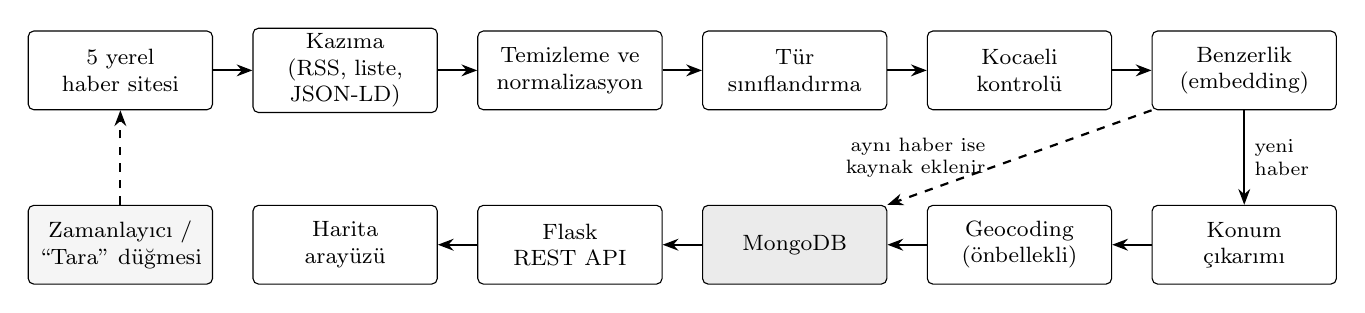
\begin{tikzpicture}[
  box/.style={draw, rounded corners=2pt, align=center, font=\footnotesize,
              minimum height=10mm, text width=22mm, inner sep=2pt},
  db/.style={box, fill=black!8},
  arr/.style={-{Stealth[length=2mm]}, thick}]
  \node[box] (siteler) {5 yerel\\haber sitesi};
  \node[box, right=5mm of siteler] (kazima) {Kazıma\\(RSS, liste,\\JSON-LD)};
  \node[box, right=5mm of kazima] (temiz) {Temizleme ve\\normalizasyon};
  \node[box, right=5mm of temiz] (sinif) {Tür\\sınıflandırma};
  \node[box, right=5mm of sinif] (yerel) {Kocaeli\\kontrolü};
  \node[box, right=5mm of yerel] (benzer) {Benzerlik\\(embedding)};
  \node[box, below=12mm of benzer] (konum) {Konum\\çıkarımı};
  \node[box, left=5mm of konum] (geo) {Geocoding\\(önbellekli)};
  \node[db, left=5mm of geo] (mongo) {MongoDB};
  \node[box, left=5mm of mongo] (api) {Flask\\REST API};
  \node[box, left=5mm of api] (harita) {Harita\\arayüzü};
  \node[box, left=5mm of harita, fill=black!4] (zaman) {Zamanlayıcı /\\``Tara'' düğmesi};
  \draw[arr] (siteler) -- (kazima);
  \draw[arr] (kazima) -- (temiz);
  \draw[arr] (temiz) -- (sinif);
  \draw[arr] (sinif) -- (yerel);
  \draw[arr] (yerel) -- (benzer);
  \draw[arr] (benzer) -- node[right, font=\scriptsize, align=left]{yeni\\haber} (konum);
  \draw[arr] (konum) -- (geo);
  \draw[arr] (geo) -- (mongo);
  \draw[arr] (mongo) -- (api);
  \draw[arr] (api) -- (harita);
  \draw[arr, dashed] (zaman.north) -- (siteler.south);
  \draw[arr, dashed] (benzer.south west) -- node[pos=0.5, left=3mm, align=right, font=\scriptsize]
        {aynı haber ise\\kaynak eklenir} (mongo.north east);
\end{tikzpicture}
\caption{Sistemin işlem hattı. Her haber soldan sağa adımlardan geçer; elenen
haberler nedeniyle birlikte \texttt{processed\_urls} koleksiyonuna yazılır.}
\label{fig:mimari}
\end{figure*}

\begin{table}[!t]
\caption{MONGODB KOLEKSİYONLARI}
\label{tab:koleksiyon}
\centering\footnotesize
\begin{tabular}{@{}p{0.27\columnwidth}p{0.66\columnwidth}@{}}
\toprule
\textbf{Koleksiyon} & \textbf{İçerik} \\
\midrule
\texttt{news} & Haritada gösterilen haberler: tür, başlık, içerik, konum metni,
enlem/boylam, yayın tarihi, kaynak listesi, sınıflandırma puanları \\
\texttt{processed\_urls} & İncelenen her linkin sonucu ve elenme nedeni \\
\texttt{geocache} & Geocoding önbelleği (servis + sorgu) \\
\texttt{scrape\_runs} & Her tarama çalışmasının özeti \\
\bottomrule
\end{tabular}
\end{table}

% =====================================================================
\section{WEB KAZIMA MODÜLÜ}\label{sec:kazima}

\subsection{Kaynak Sitelerin Yapısı}
Proje dokümanında verilen beş sitenin yapısı incelendiğinde, Çağdaş Kocaeli,
Özgür Kocaeli, Ses Kocaeli ve Bizim Yaka'nın aynı içerik yönetim sistemini
kullandığı görülmüştür. Bu sitelerde haber adresleri
\texttt{/haber/\{id\}/\{başlık\}} kalıbındadır. Bu yüzden dört site için tek bir
ortak sınıf yazılmış, siteye özel yalnızca ad ve adres bilgisi alt sınıflarda
tanımlanmıştır. Yeni Kocaeli farklı bir yapıya
(\texttt{/haber/\{kategori\}/\{başlık\}/\{id\}.html}) sahip olduğu için ayrı bir
sınıfla ele alınmıştır.

\subsection{Link Keşfi}
Haber linkleri üç kaynaktan toplanır: RSS beslemeleri, site haritaları ve liste
sayfaları (ana sayfa, kategori sayfaları ve ``kaza'', ``yangın'' gibi etiket
sayfaları). Bulunan her link, sitenin haber adresi kalıbına karşılık gelen bir
düzenli ifadeyle kontrol edilir; menü, yazar ve reklam linkleri bu şekilde
elenir. Linkler sorgu parametrelerinden arındırılarak tek biçime getirilir.

\subsection{Son Üç Gün Kuralı}
RSS beslemesinden yayın tarihi gelen eski haberler hiç indirilmez. Tarihi
bilinmeyen linkler için şu gözlemden yararlanılmıştır: Bu sitelerde haber
numaraları zamanla artmaktadır. Linkler numaraya göre yeniden eskiye sıralanır;
arka arkaya 12 eski habere rastlandığında o sitenin taraması durdurulur. Gün
sayısı ayarlanabilir; otomatik tarama son üç günü kapsar.

\subsection{Haber Sayfasının Ayrıştırılması}
Haber siteleri, arama motorları için sayfalarına \texttt{schema.org}
\emph{NewsArticle}~\cite{schemaorg} biçiminde yapılandırılmış veri (JSON-LD)
eklemektedir. Başlık, yayın tarihi ve haber metni öncelikle bu veriden okunur.
Bulunamazsa sırasıyla Open Graph meta etiketleri, \texttt{<time>} etiketi ve
sayfadaki ``22 Eylül 2026 16:18'' gibi Türkçe tarih ifadeleri denenir. Haber
gövdesi için önce siteye özel CSS seçicileri, bulunamazsa doğrudan altında en çok
paragraf metni bulunan HTML bloğu kullanılır. Tüm tarihler UTC olarak saklanır;
saat dilimi belirtilmemişse Türkiye saati varsayılır.

\subsection{Otomatik ve Tekrar Tetiklenebilir Çalışma}
Tarama, uygulama açıldıktan birkaç saniye sonra ve sonrasında düzenli
aralıklarla (varsayılan 60~dakika) APScheduler ile otomatik olarak başlatılır.
Ayrıca arayüzdeki ``Haberleri tara'' düğmesi istenen gün sayısı için taramayı
elle başlatır. Bir kilit mekanizması, iki taramanın aynı anda çalışmasını
engeller.

İstekler arasında bekleme süresi bırakılır ve ağ hatalarında istek üç kez
tekrarlanır. Sitelerin bot koruması devreye girerse (HTTP 403/429/503), istek
gerçek bir tarayıcının TLS parmak izini taklit eden \texttt{curl\_cffi}
kütüphanesiyle yeniden denenir.

% =====================================================================
\section{VERİ TEMİZLEME VE ÖN İŞLEME}
Proje dokümanında istenen her ön işleme adımı ayrı bir fonksiyon olarak
gerçekleştirilmiştir:
\begin{enumerate}
\item \emph{HTML etiket temizliği:} Betik, stil, \texttt{iframe}, menü, görsel ve
benzeri etiketler tamamen silinir; paragraflar metin satırlarına dönüştürülür.
\item \emph{Reklam ve alakasız bölümler:} \texttt{class} veya \texttt{id}
değerinde ``reklam'', ``ilgili'', ``paylaş'', ``yorum'' gibi ifadeler geçen
bloklar silinir. Ana haber kapsayıcısının yanlışlıkla silinmemesi için, sayfadaki
paragraf metninin \%60'ından fazlasını içeren bloklar korunur. Ayrıca ``ABONE OL'',
ajans adları ve görsel altında tekrarlanan başlık gibi kalıp satırlar çıkarılır.
\item \emph{Metin normalizasyonu:} Unicode birleştirme (NFC) uygulanır; farklı
tırnak, kesme ve tire karakterleri tek biçime indirilir.
\item \emph{Özel karakter temizliği:} Harf, rakam ve temel noktalama dışındaki
karakterler (emoji vb.) silinir; tekrarlanan noktalama sadeleştirilir.
\item \emph{Fazla boşluk temizliği:} Ardışık boşluklar tek boşluğa indirilir.
\end{enumerate}

Analiz için metnin ayrıca küçük harfli ve noktalamasız bir sürümü üretilir.
Burada Türkçeye özgü bir sorun çözülmüştür: Python'un \texttt{lower()}
fonksiyonu ``İ'' harfini tek bir ``i'' yerine ``i'' ve birleşik nokta
karakterinden oluşan iki karaktere, ``I'' harfini de ``ı'' yerine ``i'' harfine
dönüştürür. Bu yüzden büyük/küçük harf
dönüşümü Türkçe kurallarına göre ayrıca yazılmıştır.

% =====================================================================
\section{HABER TÜRÜ SINIFLANDIRMA}

\subsection{Yöntem}
Sınıflandırma, ağırlıklı anahtar kelime puanlamasına dayanır. Her tür için
anahtar kelimeler ve ağırlıkları Tablo~\ref{tab:anahtar}'de verilmiştir.
Ağırlıklar dört düzeydedir: türü neredeyse kesin gösteren ifadeler (+4/+5,
ör. ``trafik kaza''), güçlü ipuçları (+3, ör. ``çarpıştı''), zayıf ipuçları
(+1/+2, ör. ``sürücü'') ve yanlış eşleşmeleri bastıran negatif kelimeler (ör.
``iş kazası'' için $-6$, ``su kesintisi'' için $-5$).

Kelimeler varsayılan olarak kök biçiminde eşleşir; böylece ``yangın'' kelimesi
``yangında'' ve ``yangını'' biçimlerini de bulur. Kök eşleşmenin yanlış sonuç
verdiği kelimeler (ör. ``kaza'' kökü ``kazanç'' kelimesini de bulur) yalnızca tam
kelime olarak eşleşecek şekilde işaretlenmiştir. Başlıktaki eşleşmeler iki kat
sayılır ve aynı kelime en fazla üç kez puanlanır. Yöntem Algoritma~\ref{alg:sinif}'de
özetlenmiştir.

\begin{algorithm}[!t]
\caption{Haber türü sınıflandırma}
\label{alg:sinif}
\footnotesize
\begin{algorithmic}[1]
\Require başlık $b$, içerik $m$, kelime tablosu $K$
\Ensure tür veya \textsc{yok}
\State $b', m' \gets$ normalize$(b)$, normalize$(m)$
\State $p[t] \gets 0$ (her tür için);\ \ $G \gets \emptyset$
\For{tür $t$ ve $(k, w) \in K[t]$}
  \State $p[t] \mathrel{+}= w \cdot (2\cdot\text{say}(k,b') + \text{say}(k,m'))$
  \If{$k$ eşleşti ve $w \ge 3$} \State $G \gets G \cup \{t\}$ \EndIf
\EndFor
\State $A \gets \{t \mid t \in G,\ p[t] \ge 4\}$
\If{$A = \emptyset$} \Return \textsc{yok} \EndIf
\State $p^* \gets \max_{t\in A} p[t]$;\ \ $C \gets \{t \in A \mid p[t] \ge 0{,}6\,p^*\}$
\State \Return $C$ içinde öncelik sırası en yüksek tür
\end{algorithmic}
\end{algorithm}

\subsection{Güçlü Kelime Şartı}
Gerçek verilerle yapılan ilk denemede, ``şüpheli'', ``yakalandı'' ve
``tutuklandı'' gibi zayıf kelimelerin toplamının eşiği aştığı ve bir cinayet
haberinin ``Hırsızlık'' olarak sınıflandırıldığı görülmüştür. Bu yüzden bir
türün seçilebilmesi için, o türün ağırlığı en az 3 olan bir kelimesinin haberde
geçmesi şartı eklenmiştir ($G$ kümesi). Zayıf kelimeler artık yalnızca
destekleyici rol oynamaktadır.

\subsection{Öncelik Sırası}
Bir haber birden fazla türe uyuyorsa (puanı en yüksek puanın \%60'ına ulaşan
türler), şu öncelik sırası uygulanır: Yangın $>$ Trafik Kazası $>$ Hırsızlık $>$
Elektrik Kesintisi $>$ Kültürel Etkinlikler. Sıralamada can ve mal güvenliğini en
doğrudan tehdit eden ve acil müdahale gerektiren olay önce gelir. Örneğin
``zincirleme kazada araç alev aldı'' haberinde trafik puanı daha yüksek olsa da
iki tür birlikte aday olduğunda haber ``Yangın'' olarak etiketlenir.
Sınıflandırma sonucu, tür puanları ve eşleşen kelimelerle birlikte
veritabanında saklanır.

\begin{table*}[!t]
\caption{SINIFLANDIRMADA KULLANILAN ANAHTAR KELİMELER VE AĞIRLIKLARI}
\label{tab:anahtar}
\centering\footnotesize
\begin{tabular}{@{}p{0.15\textwidth}p{0.05\textwidth}p{0.74\textwidth}@{}}
\toprule
\textbf{Haber türü} & \textbf{Ağırlık} & \textbf{Anahtar kelimeler} \\
\midrule
Yangın & +4 & yangın, küle dön, kül oldu, kundak \\
 & +3 & alevlere teslim, alev aldı, alev alev, tutuştu, söndürül, dumandan etkilen, yandı\textsuperscript{\dag} \\
 & +2 & tutuşma, söndürme, yanarak \\
 & +1 & alev, itfaiye, patlama \\
 & -2 & yangın söndürme tüpü \\
 & -5 & tatbikat \\
\midrule
Trafik Kazası & +5 & trafik kaza, zincirleme kaza \\
 & +4 & yayaya çarp \\
 & +3 & kafa kafaya, takla at, şarampol, kontrolden çık, direksiyon hakimiyet, çarpıştı, çarpışma, çarpışan, arkadan çarp, devrildi, devrilen, sürücüsü yaralandı, maddi hasar, kaza\textsuperscript{\dag}, kazada\textsuperscript{\dag}, kazaya\textsuperscript{\dag}, kazayı\textsuperscript{\dag}, kazayla\textsuperscript{\dag}, kazazede \\
 & +2 & zincirleme, bariyer, refüj, kazası\textsuperscript{\dag}, kazalar \\
 & +1 & otomobil, motosiklet, kamyon, tır\textsuperscript{\dag}, tırın\textsuperscript{\dag}, minibüs, sürücü, yaralandı, ambulans, trafik ekip, plakalı \\
 & -3 & asfalt, ihale \\
 & -4 & yol çalışma \\
 & -5 & yeni kavşak, kavşak düzenleme, kavşak çalışma \\
 & -6 & iş kaza, ağaç devril, direk devril \\
\midrule
Hırsızlık & +5 & hırsız \\
 & +4 & çalıntı, gasp, soygun, soyuldu, yankesici, kapkaç \\
 & +3 & çaldı\textsuperscript{\dag}, çaldılar, çalındı, çalınan, çalarak, çaldığı, çaldıkları \\
 & +1 & ziynet, ele geçirildi, şüpheli, gözaltına, yakalandı, tutuklandı \\
 & -3 & uyuşturucu, dolandırıcılık \\
 & -4 & usulsüzlük, rüşvet, kapı çal, kapısını çal, zil çal \\
 & -5 & öldür, cinayet, istiklal marşı \\
\midrule
Elektrik Kesintisi & +5 & elektrik kesinti, elektrikler kesil, enerji kesinti, elektrik verilemeye, elektrik verilmeye \\
 & +4 & elektrikler gitti, elektriksiz, planlı kesinti, plansız kesinti, elektrik arıza \\
 & +3 & kesinti yapılacak, kesinti uygulanacak \\
 & +2 & sedaş, karanlıkta kal \\
 & +1 & trafo, elektrik, kesinti \\
 & -3 & seçim, meclis üye \\
 & -5 & su kesinti, doğalgaz kesinti, doğal gaz kesinti, sanayi odası \\
\midrule
Kültürel Etkinlikler & +4 & konser\textsuperscript{\dag}, konseri, konserde, konsere, konserler, konserden, tiyatro, festival, dinleti, resital, kitap fuar \\
 & +3 & sergi\textsuperscript{\dag}, sergisi, sergide\textsuperscript{\dag}, sergiye\textsuperscript{\dag}, sergiler, söyleşi, müzikal, opera\textsuperscript{\dag}, operası, operada\textsuperscript{\dag}, bale\textsuperscript{\dag}, orkestra, korosu, kültür sanat, imza günü, şenlik, panayır, sanatsever, kültür ve sanat, sempozyum, resim yarışması, film gösterim, sanat etkinli \\
 & +2 & koro\textsuperscript{\dag}, kültürel, etkinlik, sahne, gösterim, sinema, şiir, sanatçı, müze, kültür merkezi, kitap okuma \\
 & +1 & gösteri, fuar, atölye, konferans \\
 & -3 & transfer, lig\textsuperscript{\dag}, aday, seçim, atama, atandı \\
 & -4 & operasyon, tutuklan, gözaltı, futbol, maç\textsuperscript{\dag}, maçı \\
 & -6 & uyuşturucu \\
\bottomrule
\end{tabular}
\par\vspace{3pt}\begin{minipage}{0.96\textwidth}\footnotesize
Kelimeler kök olarak eşleşir; Türkçe ekleriyle birlikte de bulunur (ör. \emph{yangın} $\rightarrow$ \emph{yangında}). \textsuperscript{\dag}~ile işaretli kelimeler yalnızca tam kelime olarak eşleşir (ör. \emph{kaza} eşleşir, \emph{kazanç} eşleşmez). Negatif ağırlıklar yanlış eşleşmeleri bastırır. Başlıktaki eşleşmeler 2 kat sayılır. Bir türün seçilebilmesi için haberde o türün ağırlığı en az 3 olan bir kelimesi geçmeli ve toplam puanı en az 4 olmalıdır. Puanı en yüksek puanın en az \%60'ı olan türler arasından öncelik sırasına göre seçim yapılır: Yangın $>$ Trafik Kazası $>$ Hırsızlık $>$ Elektrik Kesintisi $>$ Kültürel Etkinlikler.
\end{minipage}
\end{table*}


% =====================================================================
\section{KONUM BİLGİSİ ÇIKARIMI}\label{sec:konum}
Konum çıkarımı kural tabanlı bir yöntemle yapılır ve üç adımdan oluşur.

\subsection{Tüm Konum İfadelerinin Bulunması}
Metindeki konum ifadeleri beş seviyede aranır (Tablo~\ref{tab:seviye}). Mahalle,
cadde ve sokak için ``Mahallesi'', ``Caddesi'', ``Sokak'' gibi anahtar kelimeler
ve kısaltmaları (``Mah.'', ``Cad.'', ``Sk.'') düzenli ifadelerle bulunur. Yer
adının kendisi, anahtar kelimenin hemen solundaki büyük harfle başlayan
kelimeler geriye doğru toplanarak çıkarılır (en fazla 4--5 kelime). Bu sırada:
\begin{itemize}
\item Cümle başında büyük harfle yazılan ``Olay'', ``Kaza'', ``Böylelikle'' gibi
kelimeler addan atılır.
\item Kesme işaretli kelimeler adın dışında bırakılır (``İzmit'in Yenişehir
Mahallesi'' $\rightarrow$ ``Yenişehir Mahallesi'').
\item Başka bir ile ait adresler eklenmez (``İznik'in Sarıalan mahallesi'').
\end{itemize}

Belirli yerler için kavşak, sapak, köprü, park, stadyum, kongre merkezi, iskele
gibi 45 yer türü tanımlanmıştır. ``Hastanesi'' bu listeye bilinçli olarak
alınmamıştır, çünkü haberlerde hastane olay yerini değil, yaralının götürüldüğü
yeri belirtir (``Kocaeli Şehir Hastanesi'ne kaldırıldı''). Anahtar kelime
içermeyen ``Sekapark'', ``Ormanya'' gibi bilinen yerler için ayrıca küçük bir yer
sözlüğü kullanılır. İlçe tespitinde ``Gölcük Mahallesi'' gibi mahalle adlarının ve
``İzmit Körfezi'' gibi ifadelerin ilçe sayılmaması için ilçe adından sonra gelen
kelime de kontrol edilir.

\begin{table}[!t]
\caption{KONUM SEVİYELERİ VE GERÇEK VERİDEN ÖRNEKLER}
\label{tab:seviye}
\centering\footnotesize
\begin{tabular}{@{}c p{0.22\columnwidth} p{0.6\columnwidth}@{}}
\toprule
\textbf{Sv.} & \textbf{Tür} & \textbf{Örnek} \\
\midrule
5 & Cadde/sokak & Kavak Caddesi, Arapçeşme Mahallesi, Gebze \\
4 & Belirli yer & Kocaeli Kongre Merkezi; Akse Sapağı, Gebze \\
3 & Mahalle/köy & Çınarlı Mahallesi, Derince \\
2 & Yol & D-100 Karayolu, Körfez \\
1 & İlçe & Kartepe \\
\bottomrule
\end{tabular}
\end{table}

\subsection{Kocaeli Kontrolü}
Yerel siteler başka illerin haberlerini de yayımlamaktadır (ör. ``Bursa'nın Kestel
ilçesinde orman yangını''). Bu yüzden metindeki Kocaeli ve ilçe anılmaları ile
diğer il ve komşu ilçe (Tuzla, Sapanca, Çiftlikköy vb.) anılmaları puanlanır.
Başlık ve ilk cümle iki kat ağırlıklıdır. ``İstanbul istikametinde'' veya
``Yalova-İzmit kara yolu'' gibi yön ve güzergâh ifadeleri sayılmaz. Dış yer puanı
Kocaeli puanından yüksekse haber kapsam dışı kabul edilir. ``Aydın'' ve ``Kartal''
gibi aynı zamanda soyadı olabilen yer adları, ancak ek veya ``ili/ilçesi''
ifadesiyle birlikte geçerse sayılır.

\subsection{En Spesifik Konumdan Genele Sorgular}
Bulunan ifadelerden, en spesifikten en genele sıralı geocoding sorguları
üretilir. Örneğin ``Kocaeli'nin İzmit ilçesi Yenişehir Mahallesi Paşa Caddesi
Dönmez Sokak'ta'' ifadesi için şu sorgular üretilir:
\begin{enumerate}
\item Dönmez Sokak, Paşa Caddesi, Yenişehir Mahallesi, İzmit, Kocaeli
\item Paşa Caddesi, Yenişehir Mahallesi, İzmit, Kocaeli
\item Yenişehir Mahallesi, İzmit, Kocaeli
\item İzmit, Kocaeli
\end{enumerate}
Sorgular sırayla denenir ve doğrulamadan geçen ilk sonuç kullanılır
(Bölüm~\ref{sec:geocoding}). Böylece adres net değilse dokümanda istendiği gibi
mümkün olan en spesifik konum alınır. Hiç konum ifadesi bulunamayan haberler
haritada gösterilmez. Bulunan tüm aday ifadeler, seçilen sorgu ve denenen
sorguların sonuçları veritabanında saklanır; bu bilgiler hem arayüzdeki bilgi
penceresinden hem de bir komut satırı aracıyla görüntülenebilir.

% =====================================================================
\section{GEOCODING}\label{sec:geocoding}

\subsection{Servisler}
Sistem iki geocoding servisini destekler: Google Geocoding API~\cite{googlegeo}
ve OpenStreetMap Nominatim~\cite{nominatim}. Her iki servis de ortak bir sınıftan
türetilmiştir; önbellek, doğrulama ve sıralı deneme mantığı ortaktır, yalnızca
API çağrısı ve cevabın ortak biçime dönüştürülmesi farklıdır. Kullanılacak servis
yapılandırma dosyasından seçilir. Google API anahtarı koda yazılmaz; yalnızca
sunucu tarafında okunan ve sürüm kontrolü dışında tutulan bir \texttt{.env}
dosyasında saklanır ve tarayıcıya hiçbir zaman gönderilmez. Nominatim kullanım
kuralları gereği saniyede en fazla bir istek yapılır ve uygulama kendini tanıtan
bir \emph{User-Agent} başlığı gönderir.

\subsection{Önbellek}
Her sorgunun sonucu, servis adıyla birlikte \texttt{geocache} koleksiyonuna
yazılır. Aynı adres tekrar sorulduğunda önce bellekteki, sonra veritabanındaki
önbelleğe bakılır ve API çağrısı yapılmaz. Bulunamayan adresler de önbelleğe
yazılır; böylece bunlar için de tekrar çağrı yapılmaz. Buna karşılık kota aşımı,
ağ hatası veya geçersiz anahtar gibi geçici hatalar önbelleğe yazılmaz. Bu
durumdaki haberler sonraki taramada otomatik olarak yeniden denenir.

\subsection{Doğrulama}
Bir sonucun kabul edilmesi için şu koşulların hepsi sağlanmalıdır:
\begin{enumerate}
\item Koordinat Kocaeli'yi çevreleyen dikdörtgen içinde olmalıdır.
\item Adresin il bileşeni ``Kocaeli'' olmalıdır. Bu kontrol, dikdörtgenin içinde
kalan Sapanca gibi komşu ilçeleri eler.
\item İlçe biliniyorsa sonuçtaki ilçe ile eşleşmelidir.
\item Sonuç istenen seviyeye yeterince yakın olmalıdır. Örneğin bir mahalle
sorgusuna yalnızca ilçe merkezi dönerse sonuç reddedilir ve bir sonraki sorguya
geçilir.
\end{enumerate}
Hiçbir sorgu doğrulamadan geçemezse haber kaydedilmez. Koordinatlar hem
\texttt{lat}/\texttt{lng} alanlarında hem de MongoDB'nin coğrafi sorgularına
uygun GeoJSON biçiminde saklanır.

% =====================================================================
\section{TEKRARLI HABER TESPİTİ}\label{sec:tekrar}
Tekrar kontrolü iki katmanda yapılır.

\emph{Link düzeyi:} Aynı link ikinci kez işlenmez. Bu kural hem incelenen linklerin
kaydıyla hem de \texttt{sources.url} alanı üzerindeki tekil (unique) indeksle
veritabanı seviyesinde garanti altına alınmıştır.

\emph{İçerik düzeyi:} Farklı sitelerde yayımlanan aynı haber, cümle gömme
yöntemiyle tespit edilir. Bunun için Sentence-BERT~\cite{sbert} mimarisine dayanan
ve bilgi damıtma (knowledge distillation) ile çok dilli hale getirilmiş
\texttt{paraphrase-multilingual-MiniLM-L12-v2} modeli~\cite{multilingual,minilm}
kullanılmıştır. Model Türkçe dahil 50'den fazla dili destekler ve her metni
384~boyutlu bir vektöre dönüştürür. Haberin başlığı ve içeriğinin başı vektöre
çevrilir. Vektörler birim uzunluğa normalize edildiği için iki vektörün iç
çarpımı kosinüs benzerliğine eşittir:
\begin{equation}
\text{benzerlik}(a,b) = \frac{a \cdot b}{\lVert a \rVert\,\lVert b \rVert}
\end{equation}
Yeni haber, yayın tarihi $\pm 3$ gün içindeki kayıtlı haberlerle karşılaştırılır.
Benzerlik dokümanda belirtilen 0,90 eşiğine ulaşırsa yeni kayıt açılmaz; yeni
kaynak mevcut haberin \texttt{sources} listesine eklenir ve haritada tüm
kaynaklar listelenir. Haberler yayın tarihine göre eskiden yeniye işlendiği için
olayı ilk yayımlayan site ana kaynak olur.

% =====================================================================
\section{HARİTA VE KULLANICI ARAYÜZÜ}\label{sec:arayuz}
Arayüz, Flask üzerinde çalışan bir REST API'den veri alan tek sayfalık bir web
uygulamasıdır (Tablo~\ref{tab:api}, Şekil~\ref{fig:arayuz}). Harita Kocaeli il
merkezinde (İzmit) açılır. Her haber için türüne göre renklendirilmiş ve
sembollü bir işaret eklenir: trafik kazası için kırmızı/araç, yangın için
turuncu/alev, elektrik kesintisi için koyu lacivert/şimşek, hırsızlık için
mor/maske ve kültürel etkinlik için yeşil/nota. Aynı koordinattaki işaretlerin üst
üste binmemesi için bunlar altın açı ile oluşturulan küçük bir sarmal üzerinde
dağıtılır.

\begin{table}[!t]
\caption{REST API UÇLARI}
\label{tab:api}
\centering\footnotesize
\begin{tabular}{@{}p{0.36\columnwidth}p{0.57\columnwidth}@{}}
\toprule
\textbf{Uç} & \textbf{İşlev} \\
\midrule
\texttt{GET /api/news} & Tür, ilçe ve tarih aralığına göre filtrelenmiş haberler \\
\texttt{GET /api/news/<id>} & Tek haber; konum ve sınıflandırma ayrıntıları \\
\texttt{GET /api/stats} & Aynı filtrelerle tür başına haber sayısı \\
\texttt{POST /api/scrape} & Taramayı istenen gün sayısıyla başlatır \\
\texttt{GET /api/scrape/status} & Taramanın durumu ve son çalışmanın özeti \\
\bottomrule
\end{tabular}
\end{table}

İşarete tıklandığında açılan bilgi penceresinde başlık, tarih, konum, haberin yer
aldığı tüm kaynaklar ve haberi yeni sekmede açan ``Habere git'' düğmesi bulunur.
Açılır bir bölümde metinde tespit edilen tüm konum adayları gösterilir. Haber
türü, ilçe ve tarih aralığı filtreleri sayfa yeniden yüklenmeden çalışır:
filtre değiştiğinde API'den yeni veri alınır ve yalnızca işaretler güncellenir.
Haber metinleri dış kaynaklardan geldiği için sayfaya her zaman düz metin olarak
yazılır; böylece haber içine gizlenmiş olası zararlı kodlar çalıştırılamaz.

Harita kodu küçük bir adaptör arayüzü üzerinden yazılmıştır (işaret ekle,
işaret kaldır, bilgi penceresi aç, odaklan). Bu arayüzün biri Google Maps
JavaScript API~\cite{googlemaps}, diğeri Leaflet~\cite{leaflet} ve OpenStreetMap
için olmak üzere iki uygulaması vardır. Filtreler, haber listesi ve bilgi
penceresi her iki haritada da aynı kodla çalışır.

\begin{figure*}[!t]
\centering
\IfFileExists{arayuz.png}{%
  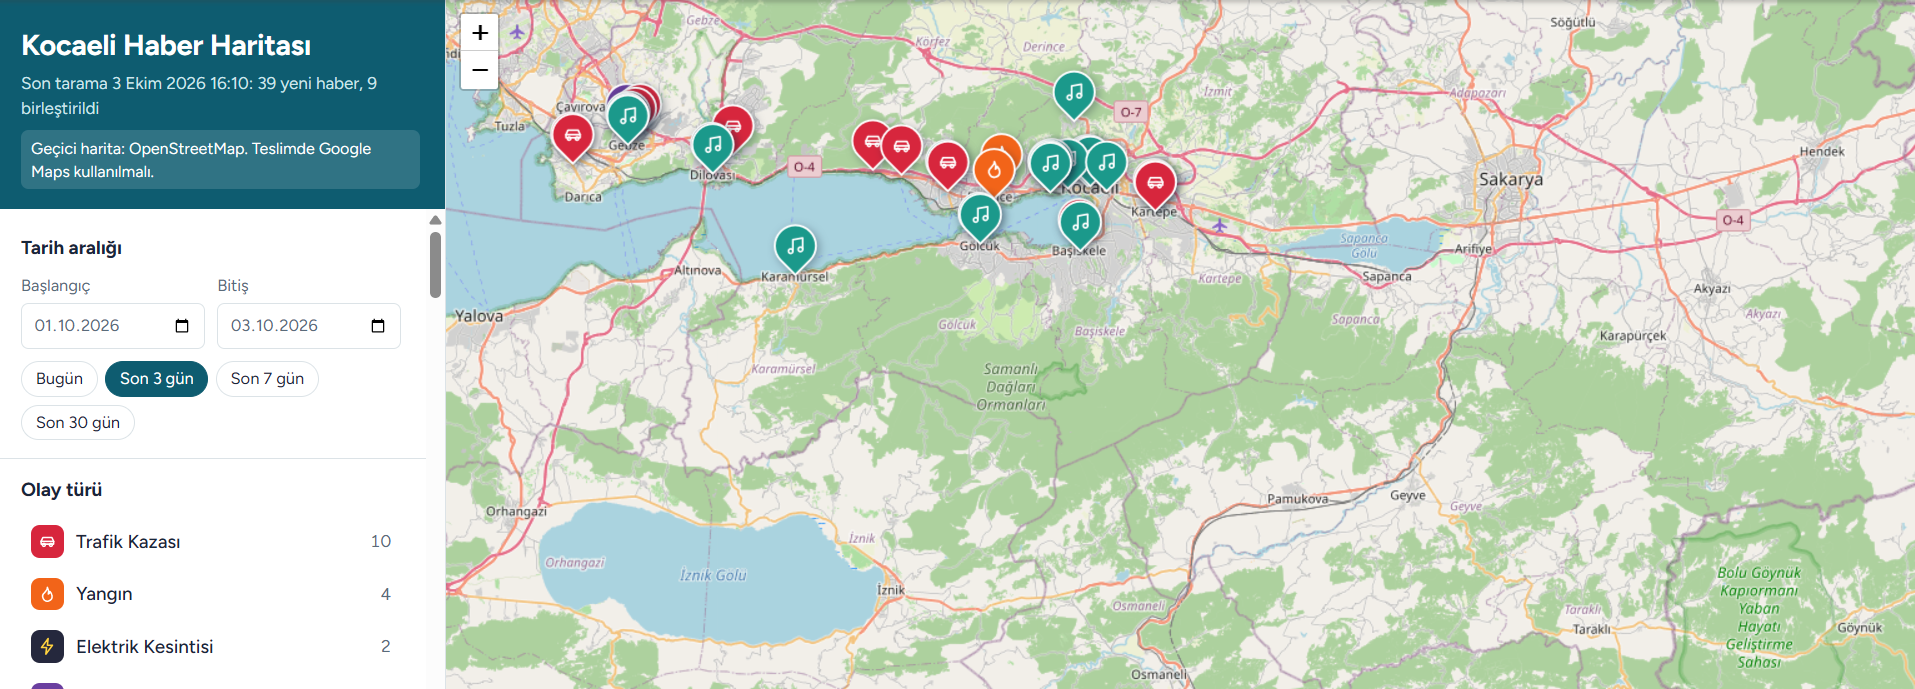
\includegraphics[width=\textwidth]{arayuz.png}%
}{%
  \fbox{\parbox[c][5cm][c]{0.9\textwidth}{\centering arayuz.png bulunamadı}}%
}
\caption{İlk taramadan sonra kullanıcı arayüzü (3~Ekim~2026). Solda tarih
aralığı, olay türü, ilçe filtreleri ve tür başına haber sayıları; sağda türüne
göre renklendirilmiş işaretlerle harita yer almaktadır. Bu ekran görüntüsü
Bölüm~\ref{sec:deney}'te açıklanan kural düzeltmelerinden önce alınmıştır.}
\label{fig:arayuz}
\end{figure*}

% =====================================================================
\section{DENEYSEL SONUÇLAR}\label{sec:deney}

\subsection{İlk Tarama}
Sistem 3~Ekim~2026 tarihinde gerçek verilerle ilk kez çalıştırılmıştır. Tarama
sonunda 39 haber kaydedilmiş, 9 haber ise başka sitelerdeki kopyalarıyla
birleştirilmiştir. Örneğin ``Kocaeli Kitap Fuarı kapılarını açtı'' haberi Ses
Kocaeli, Çağdaş Kocaeli ve Özgür Kocaeli'de yayımlanmış ve tek bir kayıtta, üç
kaynakla gösterilmiştir. Kocaeli kontrolü ise geliştirme sırasında bu sitelerden
alınan Bursa, Yalova ve İstanbul'a ait gerçek haber metinleriyle sınanmış ve bu
haberleri doğru biçimde kapsam dışı bırakmıştır.

\subsection{Sınıflandırma Hatalarının Analizi}
Kaydedilen 39 haber tek tek incelendiğinde 15'inin (\%38,5) yanlış
sınıflandırıldığı görülmüştür. Hatalar en çok Kültürel Etkinlikler (8 haber) ve
Hırsızlık (4 haber) türlerinde yoğunlaşmıştır. Hataların başlıca nedenleri ve
uygulanan çözümler Tablo~\ref{tab:hata}'da verilmiştir. Kurallar güncellendikten
sonra kayıtlı haberler, siteler yeniden taranmadan veritabanındaki metinler
üzerinden yeniden sınıflandırılmıştır. Bu işlemde 15 yanlış haberin tamamı
elenmiş, doğru sınıflandırılmış hiçbir haber yanlış türe geçmemiştir. Tür
dağılımındaki değişim Tablo~\ref{tab:dagilim}'de gösterilmiştir.

Ara aşamada güçlü kelime şartının bir yan etkisi de gözlenmiştir: ``Devrilen
motosikletin sürücüsü yaralandı'' haberi 16 puan almasına rağmen güçlü kelime
içermediği için elenmiştir. ``Devrildi'' kelimesinin ağırlığı 2'den 3'e
çıkarılarak ve ``ağaç devrildi'' gibi ifadeler negatif kelime olarak eklenerek
bu hata giderilmiştir.

\begin{table*}[!t]
\caption{GERÇEK VERİDE GÖRÜLEN SINIFLANDIRMA HATALARI VE ÇÖZÜMLERİ}
\label{tab:hata}
\centering\footnotesize
\begin{tabular}{@{}>{\raggedright\arraybackslash}p{0.26\textwidth}>{\raggedright\arraybackslash}p{0.10\textwidth}>{\raggedright\arraybackslash}p{0.28\textwidth}>{\raggedright\arraybackslash}p{0.26\textwidth}@{}}
\toprule
\textbf{Haber} & \textbf{İlk tür} & \textbf{Neden} & \textbf{Çözüm} \\
\midrule
Kocaeli'de uyuşturucu operasyonu & Kültürel & ``opera'' kökü ``operasyon'' kelimesiyle eşleşti &
``opera'' yalnızca tam biçimleriyle eşleşir; ``operasyon'' negatif \\
Genç futbolcu Fenerbahçe'ye transfer oldu & Kültürel & ``sergi'' kökü ``performans sergiledi'' ile eşleşti &
``sergi'' tam biçimlerle eşleşir; ``futbol'', ``transfer'' negatif \\
Kardeşini öldürdü & Hırsızlık & ``şüpheli'', ``tutuklandı'' gibi zayıf kelimelerin toplamı &
Güçlü kelime şartı; ``öldür'', ``cinayet'' negatif \\
Sanayi odası meclis seçimi & Elektrik & Firma adlarındaki ``elektrik'', ``trafo'' &
``sanayi odası'', ``seçim'' negatif \\
Darıca'ya yeni kavşak yapılacak & Trafik & ``kazaların önüne geçmek'' ifadesi &
``yeni kavşak'', ``ihale'' negatif \\
Milletvekili mağdurları dinledi & Hırsızlık & ``çalındı'' kelimesinin mecaz anlamı &
Ağırlık 4\,$\rightarrow$\,3 (tek başına eşiği aşamaz) \\
\bottomrule
\end{tabular}
\end{table*}

\begin{table}[!t]
\caption{TÜR DAĞILIMI: İLK SÜRÜM VE GÜNCELLENMİŞ KURALLAR}
\label{tab:dagilim}
\centering\footnotesize
\begin{tabular}{@{}lrr@{}}
\toprule
\textbf{Tür} & \textbf{İlk sürüm} & \textbf{Güncel} \\
\midrule
Trafik Kazası & 10 & 8 \\
Yangın & 4 & 4 \\
Elektrik Kesintisi & 2 & 1 \\
Hırsızlık & 4 & 0 \\
Kültürel Etkinlikler & 19 & 11 \\
\midrule
Toplam & 39 & 24 \\
\bottomrule
\end{tabular}
\end{table}

Güncellenmiş kurallarla Hırsızlık türünde haber kalmamıştır. İlk sürümde bu türde
görünen dört haberin hiçbirinin gerçekte bir hırsızlık olayı olmadığı (cinayet,
uyuşturucu, usulsüzlük ve bir siyasi ziyaret haberi) görülmüştür; dolayısıyla
boş kategori, inceleme döneminde bu türde haber yayımlanmadığını yansıtmaktadır.

\subsection{Konum Çıkarımı}
Doğru sınıflandırılmış 24 haberin konum seviyeleri Tablo~\ref{tab:konumsonuc}'da
verilmiştir. Haberlerin 16'sında (\%66,7) olay yeri ilçe merkezinden daha spesifik
bulunmuştur. İlçe seviyesinde kalan haberlerin bir kısmında metinde daha spesifik
bir konum geçmemekte, bir kısmında ise metinde geçen spesifik yer servis
tarafından bulunamamıştır. Örneğin ``Çınarlı Kartopu Sokak'' bulunamadığında
sistem bir üst seviyeye düşerek ``Çınarlı Mahallesi, Derince'' sonucunu
kullanmıştır.

\begin{table}[!t]
\caption{24 HABERDE BULUNAN KONUM SEVİYELERİ}
\label{tab:konumsonuc}
\centering\footnotesize
\begin{tabular}{@{}lrr@{}}
\toprule
\textbf{Seviye} & \textbf{Haber} & \textbf{Oran} \\
\midrule
Cadde/sokak & 6 & \%25,0 \\
Belirli yer & 7 & \%29,2 \\
Mahalle & 3 & \%12,5 \\
İlçe & 8 & \%33,3 \\
\bottomrule
\end{tabular}
\end{table}

\subsection{Tekrarlı Haber Tespitinin Sınırı}
6~Ekim~2026 tarihli taramada, aynı kazayı farklı sözcüklerle aktaran iki haberin
(``Büyükşehir'i kahreden kaza\ldots'' ve ``UlaşımPark şoförü kazada ağır
yaralandı\ldots'') birleştirilmediği görülmüştür. Bu haberlerin benzerliği \%90
eşiğinin altında kalmıştır. Eşiğin düşürülmesi bu tür eşleşmeleri yakalayabilir,
ancak farklı olayların yanlışlıkla birleştirilme riskini artırır. Eşik, proje
dokümanında belirtilen değerde bırakılmıştır.

\subsection{Otomatik Testler}
Sistem için 62 otomatik test yazılmıştır. Testler temizleme, sınıflandırma,
konum çıkarımı, sayfa ayrıştırma, geocoding, işlem hattı ve API uçlarını
kapsamaktadır. Gerçek taramada bulunan her hata ayrıca bir test
örneğine dönüştürülmüştür; böylece ileride yapılacak değişikliklerin aynı hatayı
yeniden ortaya çıkarması engellenmiştir. Testler gerçek veritabanı ve dış servis gerektirmeden,
sahte (mock) bileşenlerle çalışır.

% =====================================================================
\section{KARŞILAŞILAN SORUNLAR VE ÇÖZÜMLER}\label{sec:sorunlar}
\emph{Ulusal haberler:} Yerel siteler başka illerin haberlerini de
yayımlamaktadır. Bu sorun, yön ifadelerini dışlayan puanlamalı Kocaeli kontrolü
ve geocoding sonucundaki il doğrulamasıyla çözülmüştür.

\emph{Türkçenin eklemeli yapısı:} Kök eşleşme, ekleri yakalamak için gereklidir;
ancak ``opera/operasyon'', ``sergi/sergiledi'', ``konser/konserve'' gibi
tuzaklar oluşturmuştur. Bu kelimeler yalnızca belirli biçimleriyle eşleşecek
şekilde tanımlanmıştır. Ünsüz yumuşaması da (``verilemeyecek'' $\rightarrow$
``verilemeyeceği'') kelimelerin kaçırılmasına yol açtığı için ilgili kelimeler
yumuşayan harften önce kesilmiştir (``elektrik verilemeye'').

\emph{Çok anlamlılık:} ``Çalındı'' kelimesi hırsızlık dışında ``kapı çalındı'',
``İstiklal Marşı çalındı'' veya mecazi olarak ``emeğimiz çalındı'' anlamlarında da
kullanılmaktadır. Bu, anahtar kelime tabanlı yöntemin temel sınırlarından birini
göstermektedir.

\emph{Bot koruması:} Bazı siteler otomatik istekleri engellemiştir. Gerçek bir
tarayıcıya benzer istek başlıkları, istekler arası bekleme ve tarayıcı TLS parmak
izini taklit eden yedek bir istemci kullanılmıştır.

\emph{Ödeme yöntemi:} Google Cloud faturalandırması yalnızca uluslararası geçerli
ve ön ödemeli olmayan kartları kabul etmektedir. Geliştirme sürecinde bu koşulu
sağlayan bir kart bulunamadığı için servis seçimi soyutlanmış ve testler
OpenStreetMap servisleriyle yapılmıştır. Google API anahtarları tanımlandığında
sistem herhangi bir kod değişikliği olmadan Google servislerine geçmektedir.

% =====================================================================
\section{SONUÇ VE GELECEK ÇALIŞMALAR}\label{sec:sonuc}
Bu çalışmada beş yerel haber sitesinden haber toplayan, sınıflandıran, konumlandıran,
tekrarları birleştiren ve harita üzerinde sunan uçtan uca bir sistem
geliştirilmiştir. Gerçek verilerle yapılan deneyler, kural tabanlı yöntemlerin
doğru tasarlandığında yüksek açıklanabilirlik sağladığını, ancak dilin
eklemeli ve çok anlamlı yapısına karşı dikkatli bir hata analizi gerektirdiğini
göstermiştir. Her kararın (eşleşen kelimeler, puanlar, denenen adresler)
veritabanında saklanması, bu hata analizini mümkün kılmıştır.

Gelecek çalışmalarda anahtar kelime yönteminin, etiketli haberlerle ince ayar
yapılmış Türkçe bir dil modeliyle desteklenmesi planlanabilir. Konum çıkarımı
Türkçe adlandırılmış varlık tanıma (NER) modelleriyle güçlendirilebilir. Ayrıca
``Kocaeli'nin 6 ilçesi elektriksiz kalacak'' gibi birden fazla yeri ilgilendiren
haberler için birden fazla işaret gösterilmesi ve benzerlik eşiğinin etiketli bir
veri kümesi üzerinde kalibre edilmesi sistemi iyileştirecektir.

% =====================================================================
\begin{thebibliography}{99}
\bibitem{sbert}
N.~Reimers and I.~Gurevych, ``Sentence-BERT: Sentence embeddings using Siamese
BERT-networks,'' in \emph{Proc. Conf. Empirical Methods in Natural Language
Processing (EMNLP-IJCNLP)}, Hong Kong, 2019, pp. 3982--3992.

\bibitem{multilingual}
N.~Reimers and I.~Gurevych, ``Making monolingual sentence embeddings multilingual
using knowledge distillation,'' in \emph{Proc. Conf. Empirical Methods in Natural
Language Processing (EMNLP)}, 2020, pp. 4512--4525.

\bibitem{minilm}
Hugging Face, ``sentence-transformers/paraphrase-multilingual-MiniLM-L12-v2,''
model kartı. [Çevrimiçi]. Erişim: \url{https://huggingface.co/sentence-transformers/paraphrase-multilingual-MiniLM-L12-v2}

\bibitem{mongodb}
MongoDB, Inc., ``MongoDB documentation.'' [Çevrimiçi]. Erişim:
\url{https://www.mongodb.com/docs/}

\bibitem{googlegeo}
Google, ``Geocoding API overview.'' [Çevrimiçi]. Erişim:
\url{https://developers.google.com/maps/documentation/geocoding/overview}

\bibitem{googlemaps}
Google, ``Maps JavaScript API.'' [Çevrimiçi]. Erişim:
\url{https://developers.google.com/maps/documentation/javascript}

\bibitem{nominatim}
OpenStreetMap Foundation, ``Nominatim usage policy.'' [Çevrimiçi]. Erişim:
\url{https://operations.osmfoundation.org/policies/nominatim/}

\bibitem{leaflet}
V.~Agafonkin, ``Leaflet: An open-source JavaScript library for interactive
maps.'' [Çevrimiçi]. Erişim: \url{https://leafletjs.com/}

\bibitem{bs4}
L.~Richardson, ``Beautiful Soup documentation.'' [Çevrimiçi]. Erişim:
\url{https://www.crummy.com/software/BeautifulSoup/bs4/doc/}

\bibitem{flask}
Pallets, ``Flask documentation.'' [Çevrimiçi]. Erişim:
\url{https://flask.palletsprojects.com/}

\bibitem{apscheduler}
A.~Grönholm, ``Advanced Python Scheduler (APScheduler).'' [Çevrimiçi]. Erişim:
\url{https://apscheduler.readthedocs.io/}

\bibitem{schemaorg}
Schema.org, ``NewsArticle.'' [Çevrimiçi]. Erişim:
\url{https://schema.org/NewsArticle}
\end{thebibliography}

\end{document}

